\documentclass[11pt]{article}
\usepackage{icmlko}
\begin{document}

\title{내가 오늘 넣은 것을 오늘 뺐다 --- 그리고 판이 올랐다}
\author{월드모델 실험실}
\date{노트 432 · 2026년 8월 4일}
\maketitle

\begin{abstract}
노트 431이 ``한 짝의 $1.000$ 이 열한 짝에서 $3/11$ 이 된다''를 보이고
스스로에게 숙제를 냈다 --- \emph{이번 사이클에 짝 둘로 채택한 것을 열한 짝으로
다시 봐라.} 둘이었다.

\begin{center}
\begin{tabular}{lrr}
\hline
채택 & 짝 둘 근거 & LODO 열한 짝 \\
\hline
lr $0.10$ (노트 427) & 앱 $+0.0046$ · KR $+0.0121$ & $\mathbf{4/11}$, 평균 $-0.0031$ \\
깊이 $12$ (노트 426) & 앱 $+0.0292$ · KR $+0.0267$ & $\mathbf{4/11}$, 평균 $-0.0046$ \\
\hline
\end{tabular}
\end{center}

\textbf{둘 다 부호가 뒤집혔다.} 그리고 둘의 처지가 다르다.

\textbf{깊이 $12$ 는 뺐다.} 노트 426이 그것을 넣은 근거는 \emph{오직 전이}였다
--- 판은 $-0.0018 \cdot 2/12$ 로 반대했는데 안 본 도메인 둘이 확실히 샀기
때문이었다. 그 근거가 사라졌고 판은 여전히 반대다. \textbf{근거가 없으면
빼는 것이 맞다.}

\textbf{lr $0.10$ 은 남겼다.} 다만 \textbf{이유가 바뀌었다} --- 이제 전이가
아니라 판이 근거다. \textbf{노트 427의 ``lr $0.10$ 이 전이를 산다''를
물린다.}

그리고 되돌리자 판이 올랐다: $0.4742 \to \mathbf{0.4766 \pm 0.0008}$ ---
이번 사이클에 잰 네 구성 중 제일 높다.
\end{abstract}

\section{두 짝은 집 밖이고 LODO 는 집안이다}

$+0.0280$ 이 $-0.0046$ 이 되는 것은 잡음으로 보기엔 크다. 한 가지 눈에
띄는 차이가 있다 --- KR 만화와 비게임 앱은 \textbf{수집 밖}이다(다른 나라 ·
다른 매체). LODO 열하나는 \textbf{집안}이다. 깊이를 올리는 것이 먼 손님에게
이롭고 집안 손님에게 해로울 수는 있다.

\textbf{짓지 않는다.} 노트 430이 이미 ``같은 수집이라고 친한 손님이 아니다''를
보였고(열한 중 여섯이 KR 만화보다 낮았다), 그렇다면 집 안팎이라는 구분도
그렇게 깔끔하지 않다. 지금 말할 수 있는 것은 \textbf{두 자로 잰 값이 다르다}는
사실뿐이고, 열한 짝 쪽이 표본이 크다.

\section{내 사전 등록에 흠이 있었다}

lr 감사에 이렇게 적었다 --- \emph{$4$--$7$ 이면 판이 정한다 $\to$ 판은
유지 쪽이니 유지.} 그런데 \textbf{이미 채택한 뒤라 ``유지''가 lr $0.10$ 을
뜻하게 됐다.} 안 넣었더라면 같은 말이 lr $0.06$ 을 뜻했을 것이다.

\begin{center}
\textbf{되돌림 조항은 ``유지''라 쓰지 말고 이전 상태를 이름으로 적는다.}
\end{center}

깊이 쪽은 그 함정을 안 밟았다 --- ``$\le 3$ 이면 되돌림(깊이 6)''이라 이름을
적어 뒀다. 그래서 $4/11$ 을 보고도 판까지 따져 뺄 수 있었다.

\section{남는 것}

\begin{center}
\begin{tabular}{lr}
\hline
구성 & 판 \\
\hline
깊이12 · lr$.06$ & $0.4714$ \\
깊이6 · lr$.06$ & $0.4726$ \\
깊이12 · lr$.10$ & $0.4742$ \\
\textbf{깊이6 · lr$.10$} & $\mathbf{0.4766}$ \\
\hline
\end{tabular}
\end{center}

\textbf{되돌림이 판을 올렸다.} 깊이 12 는 판에서도 전이에서도 값이 아니었다
--- 두 짝만 그렇게 말했다.

\begin{tabular}{lp{7.0cm}}
\hline
grp · gen & 이 사이클의 나머지 채택 둘도 열한 짝으로 봐야 한다. grp 는 짝
둘에서 $+0.2950 / +0.1053$ 으로 워낙 커서 뒤집힐 것 같진 않지만 \textbf{그
말을 깊이에도 했었다} \\
집 안팎 & 먼 손님과 집안 손님이 다른 답을 하는지 --- 세 번째 종류의 짝이
있어야 잰다 \\
LODO 씨앗 & 셋이다. 짝 둘 시절의 여덟보다 얇다 \\
\hline
\end{tabular}

\begin{figure}[h]
\centering
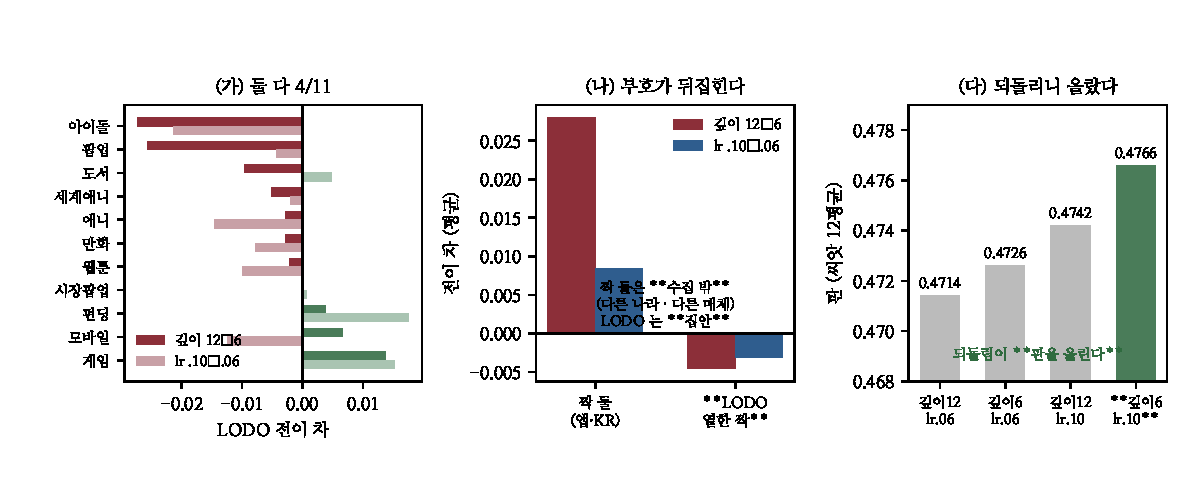
\includegraphics[width=\textwidth]{figs/fig432.pdf}
\caption{(가) 두 채택 다 $4/11$. (나) 짝 둘과 열한 짝이 부호가 반대다.
(다) 되돌리니 판이 네 구성 중 제일 높아졌다.}
\end{figure}

\end{document}
